\hypertarget{framework}{%
\section{\texorpdfstring{\href{http://en.wikipedia.org/wiki/Software_framework}{Framework}}{Framework}}\label{framework}}

\begin{itemize}
\tightlist
\item
  Fonctionnalités similaires pour de nombreuses applis
\item
  Composants de haut-niveau réutilisables (faible couplage)
\item
  Règles de codage et d'architecture
\item
  Code sûr et efficace
\item
  Facilite les tests et la gestion de projets complexes
\item
  Utilisation de Design Patterns dès que possible
\item
  Comportement par défaut
\item
  Extensible
\item
  Principe d'inversion de contrôle
\end{itemize}

Différences entre framework et library sur
\href{http://stackoverflow.com/questions/148747/what-is-the-difference-between-a-framework-and-a-library}{Stack
Overflow} ou
\href{http://www.artima.com/forums/flat.jsp?forum=106\&thread=152104}{artima
developper}.

\hypertarget{design-patterns-et-webdev}{%
\section{Design Patterns et webdev}\label{design-patterns-et-webdev}}

\begin{itemize}
\tightlist
\item
  Inversion de contrôle
  (\href{http://martinfowler.com/bliki/InversionOfControl.html}{IoC})
\item
  Model View Controller

  \begin{itemize}
  \tightlist
  \item
    M : Accès aux données, logique métier
  \item
    V : Templates des pages à générer
  \item
    C : Orchestration, transfert des infos
  \end{itemize}
\item
  Front Controller

  \begin{itemize}
  \tightlist
  \item
    Traitement et dispatch des requêtes grâce aux \textbf{routes}
  \item
    (bootstrap, ré-écriture des URL, \ldots)
  \end{itemize}
\item
  \href{https://web.archive.org/web/20160316065751/http://blog.mazenod.fr/2010/01/design-pattern-mvc-zoom-sur-la-couche-modele-dal-dao-orm-crud/}{Object
  Relational Mapping}

  \begin{itemize}
  \tightlist
  \item
    Active Record, Table Data Gateway, Data Mapper, \ldots{}
  \end{itemize}
\item
  \href{http://ui-patterns.com/}{UI Patterns}
\end{itemize}

\hypertarget{mvc-for-webdev}{%
\section{MVC for webdev}\label{mvc-for-webdev}}

\begin{figure}
\centering
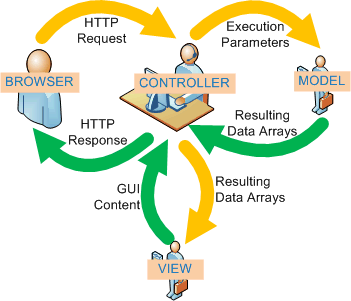
\includegraphics{src/img/mvc.png}
\caption{MVC}
\end{figure}

\hypertarget{conventions}{%
\section{Conventions}\label{conventions}}

\begin{itemize}
\tightlist
\item
  Nommage

  \begin{itemize}
  \tightlist
  \item
    Classes
  \item
    Base de données
  \item
    Fichiers et dossiers
  \end{itemize}
\item
  ROUTES :
  \textenglish{\texttt{http://app.host.tld/controller/action{[}/key/val{]}}}
\item
  Arborescence :

  \begin{itemize}
  \tightlist
  \item
    Imposée ou libre selon frameworks
  \item
    Pas de code (minimum) sous la racine web
  \end{itemize}
\item
  Conventions obligatoires ou non, mais RECOMMANDEES dans tous les cas
\end{itemize}

\hypertarget{bonnes-pratiques}{%
\section{Bonnes pratiques}\label{bonnes-pratiques}}

\begin{itemize}
\tightlist
\item
  Heavy Model, Light Controller
\item
  Don't Repeat Yourself
\item
  You Ain't Gonna Need It
\item
  Convention Over Configuration
\item
  Keep It Simple and Stupid
\item
  \href{https://12factor.net/}{12 factor app} -
  \href{https://12factor.net/fr/}{fr}
\end{itemize}

\hypertarget{pretty-smart-clean-formatted-url}{%
\section{Pretty ( \textbar{} smart \textbar{} clean \textbar{}
formatted) URL}\label{pretty-smart-clean-formatted-url}}

\begin{itemize}
\tightlist
\item
  Les URL doivent être explicites :

  \begin{itemize}
  \tightlist
  \item
    Manipulées par l'utilisateur
  \item
    Utilisées pour le référencement
  \end{itemize}
\item
  Cohérence avec l'implémentation MVC :
\end{itemize}

\begin{english}

\begin{verbatim}
http://app.host.tld/controller/action[/key/val]
\end{verbatim}

\end{english}

\begin{itemize}
\tightlist
\item
  Le routage (routing)

  \begin{itemize}
  \tightlist
  \item
    Le Front Controller recoit toutes les requêtes (URL rewriting)
  \item
    Il les dispatche vers les contrôleurs
  \end{itemize}
\end{itemize}

\hypertarget{smart-url-seo}{%
\section{Smart URL \& SEO}\label{smart-url-seo}}

\begin{figure}
\centering
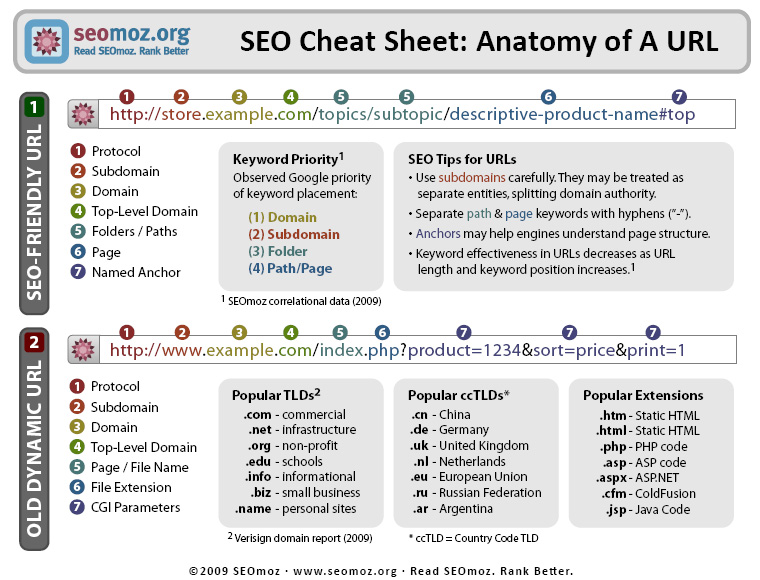
\includegraphics{src/img/anatomy-of-a-url.jpg}
\caption{SEO}
\end{figure}

\hypertarget{autres-services}{%
\section{Autres Services}\label{autres-services}}

\begin{itemize}
\tightlist
\item
  Migrations : Evolutions de la strucutre de la BDD
\item
  Tests
\item
  Génération, validation et traitement de formulaires
\item
  Authenfication, Sessions, Permissions, Roles, ACL
\item
  Pagination
\item
  I18n
\item
  Génération de code
\item
  Mail
\item
  Connecteurs aux webservices
\item
  Captchas
\item
  Loggers
\item
  \ldots{}
\end{itemize}

\hypertarget{exemple-darchitecture-laravel}{%
\section{Exemple d'architecture :
Laravel}\label{exemple-darchitecture-laravel}}

\begin{figure}
\centering
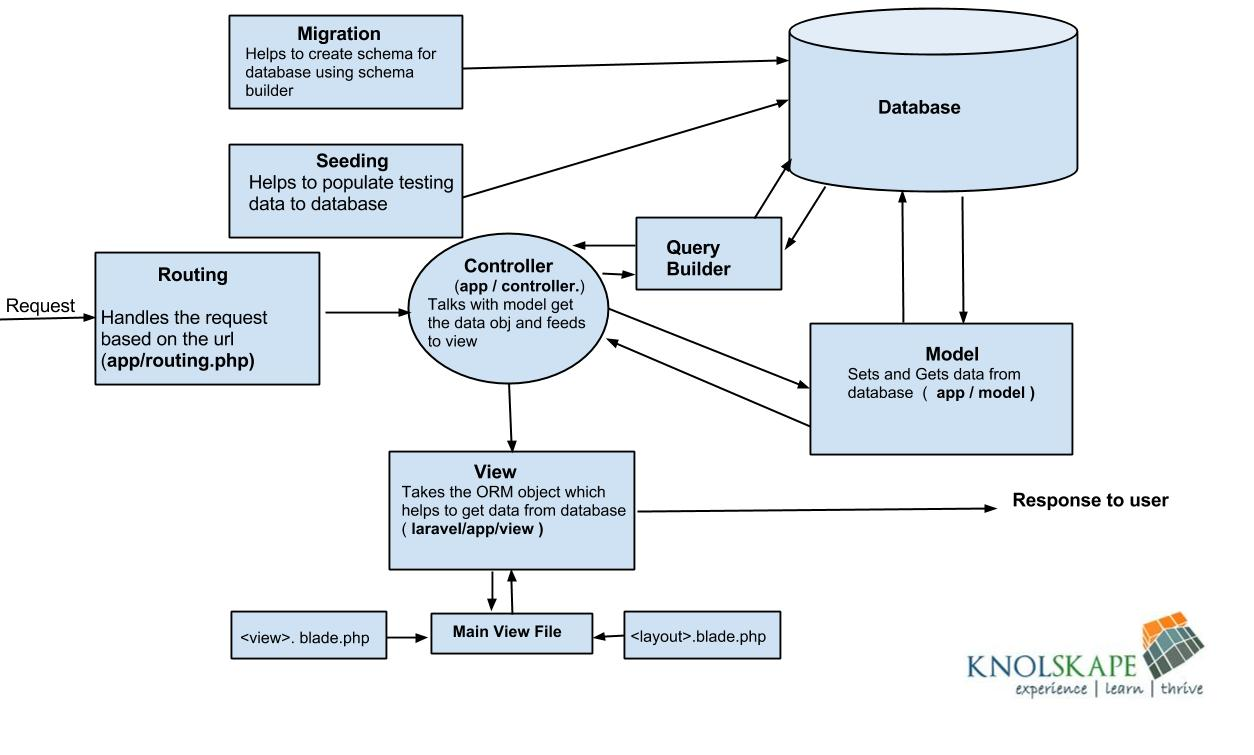
\includegraphics{src/img/laravel-architecture.jpg}
\caption{Archi}
\end{figure}

Ce schéma est clair mais pas tout à fait juste : dans Laravel, le
contrôleur récupère la page générée à partir de la vue, et c'est lui qui
renvoie le HTML (objet Response) au client.

\hypertarget{performance}{%
\section{Performance}\label{performance}}

\begin{itemize}
\tightlist
\item
  Un framework web est lent :

  \begin{itemize}
  \tightlist
  \item
    Rendu d'une page nécéssite de traverser tout le code
  \item
    Pour chaque requête toute l'appli est chargée
  \item
    Plus de code qu'une appli standalone
  \item
    Plus de requêtes
  \end{itemize}
\item
  Solutions

  \begin{itemize}
  \tightlist
  \item
    Cache de pages, d'opcode
  \item
    Jointures ORM, vues, procédures stockées
  \item
    Outils d'optimisation : YSlow, page speed, mytop
  \end{itemize}
\end{itemize}

\hypertarget{frameworks-php}{%
\section{Frameworks PHP}\label{frameworks-php}}

\begin{itemize}
\tightlist
\item
  Lesquels connaissez-vous?
\item
  Lesquels avez-vous utilisé?
\item
  Pourquoi y en a-t-il tant?
\end{itemize}

L'explication donnée par Joe Gregorio pour
\href{http://bitworking.org/news/Why_so_many_Python_web_frameworks}{le
langage Python} est : « parce que c'est facile. »

Dans les faits, cela montre également une maturité de la plateforme.

\begin{quote}
\emph{There are people who actually like programming. I don't understand
why they like programming.} Rasmus Lerdorf
\href{https://en.wikiquote.org/wiki/Rasmus_Lerdorf}{💬}
\end{quote}

\begin{itemize}
\tightlist
\item
  PHP-FI \emph{Forms Interpreter}
\item
  PHP 3, réécrit en C++
\item
  PHP 4 \emph{Zend Engine}, fausse POO
\item
  PHP 5, vraie POO
\item
  PHP 5.1, PDO
\item
  PHP 5.2, JSON
\item
  PHP 5.3, \textenglish{\texttt{goto}} et
  \textenglish{\texttt{namespace}}
\item
  PHP 5.4, \textenglish{\texttt{{[}{]}}} et \textenglish{\texttt{trait}}
\item
  PHP 5.5, \textenglish{\texttt{yield}}
\item
  \sout{PHP 6, Unicode} 💩, 🎃, 🐧
\item
  PHP 7, que du rêve!
\item
  PHP 8, JIT compilation,
  \href{https://kinsta.com/fr/blog/php-8/}{\ldots{}}
\end{itemize}

Il y a plus de vingt ans, Rasmus Lerdorf bricola un outil pour savoir
qui consultait son CV.

Zend, c'est à dire \emph{ZEev} et \emph{aNDi}, ont réécrit PHP et qui
allait devenir PHP 3 le précurseur du langage de prédilection pour créer
sur le web.

PHP a évolué depuis pour devenir ce qu'il est aujourd'hui. Sa popularité
est liée au fait qu'il est simple à mettre en œuvre, gratuit \textbf{et}
libre. Tout un tas de modules est fourni avec pour faire de l'imagerie,
des bases de données, du XML, etc.

Et plus encore sur la page
\href{http://php.net/manual/en/history.php.php}{History of PHP} et
\href{https://en.wikipedia.org/wiki/PHP}{Wikipedia: PHP}.

Les différentes moutures de PHP 7 offrent ceci, entre autres.

\begin{itemize}
\tightlist
\item
  PHP 7, performances
\item
  PHP 7.1, \textenglish{\texttt{void}}
\item
  PHP 7.2, sodium
\end{itemize}

\begin{figure}
\centering

\includegraphics{src/img/phpfig.png}
\caption{PHP Framework Interop Group}
\end{figure}

L'évolution de PHP a fait que les usagers du langage, créateur de
\emph{frameworks}, d'outils (comme
\href{http://getcomposer.org/}{\emph{Composer}}), ont senti le besoin
d'émettre des recommendations afin d'aller vers un plus interopérable.

Durant ce cours, nous allons vous embêter avec PSR-1, PSR-2 et PSR-4.

\hypertarget{quiz}{%
\section{Quiz}\label{quiz}}

Qui est qui?

\begin{figure}
\centering

\includegraphics{src/img/GandalfStaff5.jpg}
\caption{\href{http://hero.wikia.com/wiki/Gandalf}{source}}
\end{figure}

oOops, ceci n'a rien à voir avec le cours.

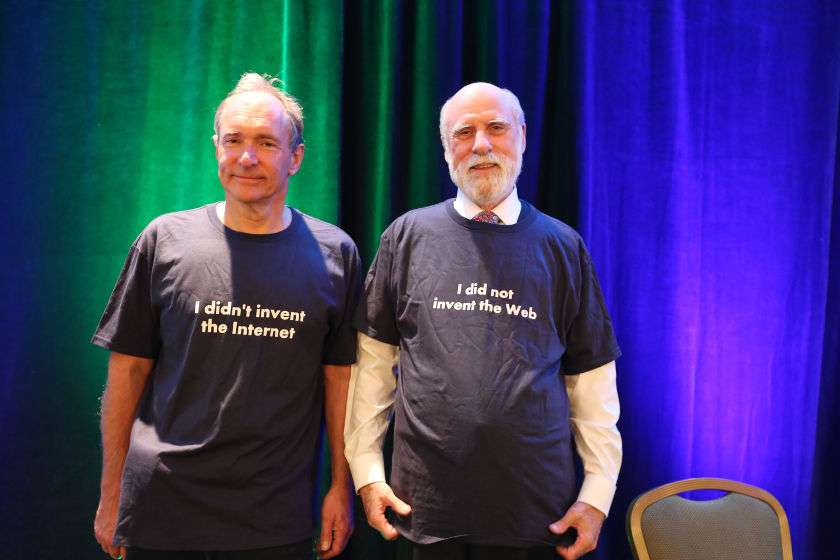
\includegraphics{src/img/0O4A8746-large.jpg}(1)

Donc, ce ne sont pas Gandalf (sans sa barbe) et Saruman mais bien Sir
Tim Berners-Lee et Vinton Cerf, responsables du (World Wide) Web et de
l'Internet.

\hypertarget{quest-ce-quinternetitcrowd}{%
\subsection{\texorpdfstring{Qu'est-ce
qu'\href{https://www.youtube.com/watch?v=iDbyYGrswtg}{Internet}
?}{Qu'est-ce qu'Internet ?}}\label{quest-ce-quinternetitcrowd}}

\begin{itemize}
\tightlist
\item
  un réseau IP
\end{itemize}

\hypertarget{quest-ce-que-le-world-wide-web}{%
\subsection{Qu'est-ce que le World Wide Web
?}\label{quest-ce-que-le-world-wide-web}}

\begin{itemize}
\tightlist
\item
  \textbf{URI/URL}, des identifiants uniques
\item
  \textbf{HTML}, un langage de publication
\item
  \textbf{HTTP}, un protocole d'échange de texte (ou \emph{HyperText})
\end{itemize}

\hypertarget{pruxe9paratifs}{%
\section{Préparatifs}\label{pruxe9paratifs}}

\href{https://github.com/HE-Arc/php-intro-framework}{https://github.com/HE-Arc/php-intro-framework/}

\begin{english}

\begin{verbatim}
$ sudo systemctl start httpd
$ cd /var/www/html
$ git clone \
> https://github.com/\
> HE-Arc/php-intro-framework

$ cd php-intro-framework
$ open http://localhost/php-intro-framework
\end{verbatim}

\end{english}

Les exemples suivant travaillent sur le code disponible dans le dépôt
\href{https://github.com/HE-Arc/php-intro-framework}{HE-Arc/php-intro-framework}.

\begin{english}

\begin{verbatim}
$ curl -v "http://he-arc.ch/?id=25"
> GET /?id=25 HTTP/1.1
> Host: he-arc.ch
>
< HTTP/1.1 200 OK
< Content-Type: text/html; charset=utf-8
<
\end{verbatim}

\end{english}

\begin{english}

\begin{Shaded}
\begin{Highlighting}[]
\DataTypeTok{\textless{}!DOCTYPE }\NormalTok{html}\DataTypeTok{\textgreater{}}
\KeywordTok{\textless{}title\textgreater{}}\NormalTok{HE{-}Arc}\KeywordTok{\textless{}/title\textgreater{}}
\KeywordTok{\textless{}p\textgreater{}}\NormalTok{Hello}
\end{Highlighting}
\end{Shaded}

\end{english}

HTTP est un protocole texte plutôt simple, jugez plutôt:

Ce que nous voyons est une connexion TCP/IP au serveur
\textenglish{\texttt{he-arc.ch}}. Une fois la connexion établie, il
envoie en texte ASCII les entêtes HTTP puis deux retours à la ligne (ce
qui correspond à une ligne vide). La requête HTTP commencent toujours
par la demande, ici
\textenglish{\texttt{GET\ /index.php?page=equipe\&id=25\ HTTP/1.1}} puis
les entêtes, ici: \textenglish{\texttt{Host:\ www.he-arc.ch}}. La
réponse du serveur est du même type, le code de réponse
(\textenglish{\texttt{HTTP/1.1\ 200\ OK}}), les entêtes, une ligne vide
puis le contenu.

La demande et les entêtes sont en US-ASCII mais le corps peut être
encodé autrement, ici c'est dit dans l'entête
\textenglish{\texttt{Content-Type:\ text/html;\ charset=utf-8}}.

\hypertarget{fait-1}{%
\subsection{Fait \#1}\label{fait-1}}

PHP parle HTTP.

Le fichier \textenglish{\texttt{index.php}} est le code PHP le plus
simple qui soit. Simple au sens du niveau de compréhension de PHP et
d'une forme de complexité.

\begin{english}

\begin{Shaded}
\begin{Highlighting}[]
\KeywordTok{\textless{}?php} \CommentTok{// 00{-}base}

\CommentTok{// Lecture de la query string \textasciigrave{}page=\textless{}XX\textgreater{}\&id=\textless{}YY\textgreater{}\textasciigrave{}.}
\KeywordTok{$page}\NormalTok{ = }\KeywordTok{$\_GET}\OtherTok{[}\StringTok{"page"}\OtherTok{]} \OtherTok{??} \KeywordTok{null}\OtherTok{;}
\KeywordTok{$id}\NormalTok{ = }\DataTypeTok{(int)} \OtherTok{(}\KeywordTok{$\_GET}\OtherTok{[}\StringTok{"id"}\OtherTok{]} \OtherTok{??} \DecValTok{0}\OtherTok{);}

\CommentTok{// Connexion à la base de données.}
\KeywordTok{$db}\NormalTok{ = }\KeywordTok{new} \KeywordTok{PDO}\OtherTok{(}\StringTok{"sqlite:../users.db"}\OtherTok{);}

\CommentTok{// Page HTML}
\KeywordTok{?\textgreater{}}
\NormalTok{\textless{}!}\KeywordTok{DOCTYPE}\NormalTok{ html\textgreater{}}
\NormalTok{\textless{}meta charset=utf}\DecValTok{{-}8}\NormalTok{\textgreater{}}
\NormalTok{\textless{}title\textgreater{}}\KeywordTok{HE}\NormalTok{{-}Arc\textless{}/title\textgreater{}}
\NormalTok{\textless{}}\OtherTok{?}\NormalTok{php}
\CommentTok{// Contenu}
\KeywordTok{if} \OtherTok{(}\StringTok{"equipe"}\NormalTok{ === }\KeywordTok{$page}\OtherTok{):}
    \KeywordTok{$query}\NormalTok{ = }\KeywordTok{$db}\NormalTok{{-}\textgreater{}query}\OtherTok{(}\StringTok{"SELECT * FROM \textasciigrave{}personnes\textasciigrave{} WHERE \textasciigrave{}id\textasciigrave{} = :id;"}\OtherTok{);}
    \KeywordTok{$query}\NormalTok{{-}\textgreater{}execute}\OtherTok{(}\NormalTok{compact}\OtherTok{(}\StringTok{\textquotesingle{}id\textquotesingle{}}\OtherTok{));}

    \KeywordTok{$personne}\NormalTok{ = }\KeywordTok{$query}\NormalTok{{-}\textgreater{}fetch}\OtherTok{(}\KeywordTok{PDO}\NormalTok{::}\KeywordTok{FETCH\_OBJ}\OtherTok{);}
\KeywordTok{?\textgreater{}}
\NormalTok{    \textless{}p\textgreater{}\textless{}a href=}\StringTok{"\textless{}?php echo }\KeywordTok{$\_SERVER}\StringTok{["}\KeywordTok{PHP\_SELF}\StringTok{"] ?\textgreater{}"}\NormalTok{\textgreater{}retour\textless{}/a\textgreater{}}
\NormalTok{    \textless{}h1\textgreater{}Équipe\textless{}/h1\textgreater{}}
\NormalTok{    \textless{}h2\textgreater{}}
\NormalTok{        \textless{}}\OtherTok{?}\NormalTok{php }\KeywordTok{echo} \KeywordTok{$personne}\NormalTok{{-}\textgreater{}prenom }\KeywordTok{?\textgreater{}}
\NormalTok{        \textless{}}\OtherTok{?}\NormalTok{php }\KeywordTok{echo} \KeywordTok{$personne}\NormalTok{{-}\textgreater{}nom }\KeywordTok{?\textgreater{}}
\NormalTok{    \textless{}/h2\textgreater{}}
\NormalTok{    \textless{}p\textgreater{}}
\NormalTok{        \textless{}img src=}\StringTok{"//www.gravatar.com/avatar/\textless{}?php}
\StringTok{            echo md5(strtolower(}\KeywordTok{$personne}\StringTok{{-}\textgreater{}email));}
\StringTok{        ?\textgreater{}"}\NormalTok{ alt=}\StringTok{"avatar"}\NormalTok{\textgreater{}}
\NormalTok{\textless{}}\OtherTok{?}\NormalTok{php}
\KeywordTok{else}\OtherTok{:}
\KeywordTok{?\textgreater{}}
\NormalTok{    \textless{}h1\textgreater{}Accueil\textless{}/h1\textgreater{}}
\NormalTok{    \textless{}ul\textgreater{}}
\NormalTok{        \textless{}li\textgreater{}\textless{}a href=}\StringTok{"?page=equipe\&amp;id=1"}\NormalTok{\textgreater{}Yoan Blanc\textless{}/a\textgreater{}}
\NormalTok{        \textless{}li\textgreater{}\textless{}a href=}\StringTok{"?page=equipe\&amp;id=2"}\NormalTok{\textgreater{}Yoan Blanc\textless{}/a\textgreater{}}
\NormalTok{    \textless{}/ul\textgreater{}}
\NormalTok{\textless{}}\OtherTok{?}\NormalTok{php}
\KeywordTok{endif}
\end{Highlighting}
\end{Shaded}

\end{english}

\hypertarget{fait-2}{%
\subsection{Fait \#2}\label{fait-2}}

PHP \textbf{est} un langage de template.

Pour preuve, il faut ouvrir une balise
\textenglish{\texttt{\textless{}?php}} pour commencer la partie code.

Avec la pratique, on a réalisé que mélanger la logique métier et celle
d'affichage n'est pas optimal car difficile à lire et maintenir.

\hypertarget{suxe9paration-muxe9tieraffichage}{%
\section{Séparation
métier/affichage}\label{suxe9paration-muxe9tieraffichage}}

\begin{english}

\begin{Shaded}
\begin{Highlighting}[]
\KeywordTok{\textless{}?php} \CommentTok{// 01{-}includes/index.php}

\CommentTok{// ...}

\KeywordTok{include} \StringTok{"templates/entete.html"}\OtherTok{;}

\KeywordTok{if} \OtherTok{(}\StringTok{"equipe"}\NormalTok{ === }\KeywordTok{$\_GET}\OtherTok{[}\StringTok{"page"}\OtherTok{])}\NormalTok{ \{}
    \CommentTok{// SELECT FROM u WHERE id=$\_GET["id"]}
    \CommentTok{// ...}
    \KeywordTok{include} \StringTok{"templates/equipe.html"}\OtherTok{;}
\NormalTok{\} }\KeywordTok{else}\NormalTok{ \{}
    \CommentTok{// ...}
    \KeywordTok{include} \StringTok{"templates/accueil.html"}\OtherTok{;}
\NormalTok{\}}
\end{Highlighting}
\end{Shaded}

\end{english}


\includegraphics{src/img/meme10.jpg}

Quel est le problème avec cette solution?

(\href{https://raw.githubusercontent.com/cyrilmanuel/picbot/e6ff24a8bfd7ee9f0514a4fd8f49b1255ef26178/picbot/Images/meme10.jpg}{Source
de l'image})

\hypertarget{suxe9curituxe9-des-templates}{%
\section{Sécurité des templates}\label{suxe9curituxe9-des-templates}}

\begin{itemize}
\tightlist
\item
  \emph{Principle of Least Privilege} (
  \href{https://en.wikipedia.org/wiki/Principle_of_least_privilege}{polp}
  )
\item
  Intégration faite par un graphiste, société externe
\end{itemize}

Dans ce le cas présent rien ne nous empêche de mettre de la logique
métier dans nos fichiers de \emph{template}, car ils sont faits de PHP
eux aussi.

\begin{english}

\begin{Shaded}
\begin{Highlighting}[]
\NormalTok{\{\# 02{-}twig/templates/collaborateur.html \#\}}
\NormalTok{\{\%{-} extends "base.html" {-}\%\}}

\NormalTok{\{\% block corps {-}\%\}}
\KeywordTok{\textless{}p\textgreater{}\textless{}a}\OtherTok{ href=}\StringTok{"?"}\KeywordTok{\textgreater{}}\NormalTok{retour}\KeywordTok{\textless{}/a\textgreater{}}
\KeywordTok{\textless{}h1\textgreater{}}\NormalTok{Équipe}\KeywordTok{\textless{}/h1\textgreater{}}
\KeywordTok{\textless{}h2\textgreater{}}
\NormalTok{  \{\{{-} personne.prenom {-}\}\}}
\NormalTok{  \{\{ personne.nom {-}\}\}}
\KeywordTok{\textless{}/h2\textgreater{}}
\KeywordTok{\textless{}p\textgreater{}\textless{}img}
\OtherTok{  src=}\StringTok{"//www.gravatar.com/avatar/}
\StringTok{  \{\{{-} personne.email | strtolower | md5 \}\}"}
\OtherTok{  alt=}\StringTok{"avatar"}\KeywordTok{\textgreater{}}
\NormalTok{\{\% endblock {-}\%\}}
\end{Highlighting}
\end{Shaded}

\end{english}

La page est réalisée avec \href{http://twig.sensiolabs.org/}{Twig}
\textless2.0. À partir de la version 2.0, il faut utiliser un
\emph{autoloader} externe, comme celui de composer (voir ci-dessous).

Le code est un poil plus propre du côté de nos \emph{templates} qui ne
peuvent plus exécuter de PHP sauf ce qu'on leur autorise, ici
\textenglish{\texttt{md5}} et \textenglish{\texttt{strtolower}}. Voir
\href{02-twig/index.php}{\textenglish{\texttt{02-twig/index.php}}}.

\begin{english}

\begin{Shaded}
\begin{Highlighting}[]
\KeywordTok{\textless{}?php} \CommentTok{// 02{-}twig}

\KeywordTok{require\_once} \StringTok{\textquotesingle{}Twig/lib/Twig/Autoloader.php\textquotesingle{}}\OtherTok{;}
\NormalTok{Twig\_Autoloader::register}\OtherTok{();}

\CommentTok{// ...}

\CommentTok{// Configuration de Twig}
\KeywordTok{$loader}\NormalTok{ = }\KeywordTok{new}\NormalTok{ Twig\_Loader\_FileSystem}\OtherTok{(}\StringTok{"templates"}\OtherTok{);}
\KeywordTok{$twig}\NormalTok{ = }\KeywordTok{new}\NormalTok{ Twig\_Environment}\OtherTok{(}\KeywordTok{$loader}\OtherTok{);}

\CommentTok{// Ajout des filtres md5 et strtolower qui sont les fonctions PHP du même nom.}
\KeywordTok{$twig}\NormalTok{{-}\textgreater{}addFilter}\OtherTok{(}\KeywordTok{new}\NormalTok{ Twig\_SimpleFilter}\OtherTok{(}\StringTok{\textquotesingle{}strtolower\textquotesingle{}}\OtherTok{,} \StringTok{\textquotesingle{}strtolower\textquotesingle{}}\OtherTok{));}
\KeywordTok{$twig}\NormalTok{{-}\textgreater{}addFilter}\OtherTok{(}\KeywordTok{new}\NormalTok{ Twig\_SimpleFilter}\OtherTok{(}\StringTok{\textquotesingle{}md5\textquotesingle{}}\OtherTok{,} \StringTok{\textquotesingle{}md5\textquotesingle{}}\OtherTok{));}

\CommentTok{// variable globale}
\KeywordTok{$titre}\NormalTok{ = }\StringTok{"HE{-}Arc"}\OtherTok{;}

\CommentTok{// Contenu}
\KeywordTok{if} \OtherTok{(}\StringTok{"equipe"}\NormalTok{ === }\KeywordTok{$page}\OtherTok{)}\NormalTok{ \{}
    \CommentTok{// ...}
    \KeywordTok{$personne}\NormalTok{ = }\CommentTok{// ...}

    \KeywordTok{echo} \KeywordTok{$twig}\NormalTok{{-}\textgreater{}render}\OtherTok{(}\StringTok{"equipe.html"}\OtherTok{,}\NormalTok{ compact}\OtherTok{(}\StringTok{"titre"}\OtherTok{,} \StringTok{"personne"}\OtherTok{));}
\NormalTok{\} }\KeywordTok{else}\NormalTok{ \{}
    \KeywordTok{$personnes}\NormalTok{ = }\CommentTok{// ...}

    \KeywordTok{echo} \KeywordTok{$twig}\NormalTok{{-}\textgreater{}render}\OtherTok{(}\StringTok{"accueil.html"}\OtherTok{,}\NormalTok{ compact}\OtherTok{(}\StringTok{"titre"}\OtherTok{,} \StringTok{"personnes"}\OtherTok{));}
\NormalTok{\}}
\end{Highlighting}
\end{Shaded}

\end{english}

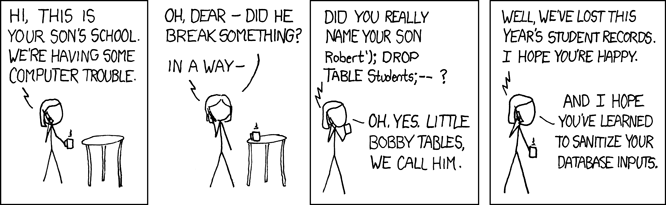
\includegraphics{src/img/exploits_of_a_mom.png} Problème d'injection
SQL.

Effectuer des requêtes MySQL à la main ou devoir connaitre tous les
champs crée beaucoup de redondance et de failles de sécurité
potentielles.

Une solution est d'ajouter une couche d'abstraction qui va cacher la
structure réelle de notre base de données et offrir une interface
orientée objet. Un \emph{Object-Relational Mapping} ou ORM(3) dans le
jargon.

\begin{english}

\begin{Shaded}
\begin{Highlighting}[]

\KeywordTok{\textless{}?php}
\CommentTok{// Ne dites plus}
\KeywordTok{$query}\NormalTok{ = }\KeywordTok{$db}\NormalTok{{-}\textgreater{}query}\OtherTok{(}
  \StringTok{"SELECT * FROM \textasciigrave{}personnes\textasciigrave{} "}\NormalTok{.}
  \StringTok{"WHERE \textasciigrave{}id\textasciigrave{} = :id;"}
\OtherTok{);}
\KeywordTok{$query}\NormalTok{{-}\textgreater{}execute}\OtherTok{(}\NormalTok{compact}\OtherTok{(}\StringTok{\textquotesingle{}id\textquotesingle{}}\OtherTok{));}
\KeywordTok{$personne}\NormalTok{ = }\KeywordTok{$query}\NormalTok{{-}\textgreater{}fetch}\OtherTok{(}\KeywordTok{PDO}\NormalTok{::}\KeywordTok{FETCH\_OBJ}\OtherTok{);}

\CommentTok{// Mais dites plutôt}

\CommentTok{//  RedBean}
\KeywordTok{$personne}\NormalTok{ = }\KeywordTok{R}\NormalTok{::load}\OtherTok{(}\StringTok{\textquotesingle{}personnes\textquotesingle{}}\OtherTok{,} \KeywordTok{$id}\OtherTok{);}
\CommentTok{// ou Doctrine}
\KeywordTok{$personne}\NormalTok{ = }\KeywordTok{$om}\NormalTok{{-}\textgreater{}find}\OtherTok{(}\StringTok{\textquotesingle{}Personne\textquotesingle{}}\OtherTok{,} \KeywordTok{$id}\OtherTok{);}
\end{Highlighting}
\end{Shaded}

\end{english}

\hypertarget{object-relational-mapping}{%
\section{\texorpdfstring{\emph{Object-Relational
Mapping}}{Object-Relational Mapping}}\label{object-relational-mapping}}

\begin{itemize}
\tightlist
\item
  \href{http://www.redbeanphp.com/}{RedBean}
\item
  \href{http://www.doctrine-project.org/}{Doctrine} (ORM, ODM)
\item
  \href{http://laravel.com/docs/master/eloquent}{Eloquent ORM}
\item
  \href{https://en.wikipedia.org/wiki/List_of_object-relational_mapping_software\#PHP}{etc.}
\end{itemize}

Une bibliothèque qui va créer ce lien entre les mondes objet et
relationnel ou document (généralement MongoDB). Il en existe toute une
foule.

\begin{english}

\begin{Shaded}
\begin{Highlighting}[]
\KeywordTok{\textless{}?php} \CommentTok{// 03{-}redbean/index.php}
\KeywordTok{require} \StringTok{\textquotesingle{}RedBean/rb.php\textquotesingle{}}\OtherTok{;}
\KeywordTok{R}\NormalTok{::setup}\OtherTok{(}\StringTok{"sqlite:../users.db"}\OtherTok{);}
\CommentTok{// ...}
\KeywordTok{if} \OtherTok{(}\StringTok{"equipe"}\NormalTok{ === }\KeywordTok{$page}\OtherTok{)}\NormalTok{ \{}
    \KeywordTok{$personne}\NormalTok{ = }\KeywordTok{R}\NormalTok{::load}\OtherTok{(}\StringTok{"personnes"}\OtherTok{,} \KeywordTok{$id}\OtherTok{);}
    \KeywordTok{echo} \KeywordTok{$twig}\NormalTok{{-}\textgreater{}render}\OtherTok{(}
        \StringTok{"equipe.html"}\OtherTok{,}
\NormalTok{        compact}\OtherTok{(}\StringTok{"titre"}\OtherTok{,} \StringTok{"personne"}\OtherTok{)}
    \OtherTok{);}
\NormalTok{\} }\KeywordTok{else}\NormalTok{ \{}
    \KeywordTok{$personnes}\NormalTok{ = }\KeywordTok{R}\NormalTok{::find}\OtherTok{(}\StringTok{"personnes"}\OtherTok{);}
    \KeywordTok{echo} \KeywordTok{$twig}\NormalTok{{-}\textgreater{}render}\OtherTok{(}
        \StringTok{"accueil.html"}\OtherTok{,}
\NormalTok{        compact}\OtherTok{(}\StringTok{"titre"}\OtherTok{,} \StringTok{"personnes"}\OtherTok{)}
    \OtherTok{);}
\NormalTok{\}}
\end{Highlighting}
\end{Shaded}

\end{english}

\hypertarget{uri-as-ui}{%
\section{URI as UI}\label{uri-as-ui}}

Pensez à Wikipedia.

Les adresses des pages font partie de l'expérience utilisateur. Un
utilisateur doit être capable d'imaginer le contenu de la page en lisant
l'URI. Certainement, ce que vous faites avant de cliquer sur un lien.

\hypertarget{comment-humaniser}{%
\subsection{Comment humaniser ?}\label{comment-humaniser}}

\begin{english}

\begin{verbatim}
  /index.php?page=equipe&id=42
\end{verbatim}

\end{english}

La personne avec l'identifiant \textenglish{\texttt{42}} aura également
un \emph{slug} unique créé à partir de son nom, ici
\textenglish{\texttt{jean-bon}}.

La solution à notre problème est de demander au serveur web de réécrire
les URL pour nous.

\hypertarget{ruxe9uxe9criture-durl}{%
\subsection{Réécriture d'URL}\label{ruxe9uxe9criture-durl}}

\begin{english}

\begin{Shaded}
\begin{Highlighting}[]
\CommentTok{\# 04{-}routes/.htaccess}

\CommentTok{\# mod\_rewrite}
\ExtensionTok{RewriteEngine}\CharTok{ }\KeywordTok{on}
\NormalTok{RewriteBase}\StringTok{ /php{-}intro{-}framework/04{-}routes/}

\NormalTok{RewriteCond}\StringTok{ \%\{REQUEST\_FILENAME\} !{-}f}
\NormalTok{RewriteCond}\StringTok{ \%\{REQUEST\_FILENAME\} !{-}d}
\NormalTok{RewriteRule}\StringTok{ \^{}(.*)$ index.php/$1 [L,QSA]}
\end{Highlighting}
\end{Shaded}

\end{english}

Apache le fait via
\href{https://httpd.apache.org/docs/current/mod/mod_rewrite.html}{\textenglish{\texttt{mod\_rewrite}}}
et Nginx
\href{http://nginx.org/en/docs/http/ngx_http_core_module.html\#try_files}{\textenglish{\texttt{try\_files}}}.

\begin{english}

\begin{Shaded}
\begin{Highlighting}[]

\CommentTok{// 04{-}routes/index.php}

\KeywordTok{$uri}\NormalTok{ = }\KeywordTok{$\_SERVER}\OtherTok{[}\StringTok{\textquotesingle{}REQUEST\_URI\textquotesingle{}}\OtherTok{],}
\KeywordTok{$matches}\NormalTok{ = }\OtherTok{[];}

\FunctionTok{preg\_match}\OtherTok{(}
    \StringTok{"\#\^{}/(?P\textless{}page\textgreater{}[\^{}/]+)/(?P\textless{}slug\textgreater{}[\^{}/]+)/?\#"}\OtherTok{,}
    \KeywordTok{$uri}\OtherTok{,}
    \KeywordTok{$matches}
\OtherTok{)} \KeywordTok{or} \KeywordTok{die}\OtherTok{(}\StringTok{\textquotesingle{}Arrrrrgh\textquotesingle{}}\OtherTok{);}

\KeywordTok{echo} \FunctionTok{call\_user\_func\_array}\OtherTok{(}
    \KeywordTok{$matches}\OtherTok{[}\StringTok{\textquotesingle{}page\textquotesingle{}}\OtherTok{],}
    \OtherTok{[}\KeywordTok{$matches}\OtherTok{[}\StringTok{\textquotesingle{}slug\textquotesingle{}}\OtherTok{]]}
\OtherTok{);}
\end{Highlighting}
\end{Shaded}

\end{english}

Le code complet va nettoyer l'URI et définir les fonction correspondant
aux pages possibles.

\hypertarget{routing}{%
\section{\texorpdfstring{\emph{Routing}}{Routing}}\label{routing}}

Lien entre les adresses (URI) et des actions dans le code.

a.k.a. the \emph{Front Controller}.

En pratique, les actions ne sont pas des fonctions mises à plat mais
sont encapsulées dans une classe qu'on nomme un contrôleur. Faire ainsi
permet de regrouper logiquement les fonctions et éviter d'utiliser
d'affreux éléments tel que \textenglish{\texttt{global}}.

\hypertarget{moduxe8le---vue---contruxf4leur}{%
\section{Modèle - Vue -
Contrôleur}\label{moduxe8le---vue---contruxf4leur}}

\begin{itemize}
\tightlist
\item
  Modèle: l'ORM qui s'occupe de notre base de données
\item
  Vue: les templates qui affiche les données
\item
  Contrôleur: une classe qui définit quoi faire en fonction des entrées
  utilisateur (URI, formulaire, etc.)
\end{itemize}

\emph{MVC}(4) vient des applications bureau et ne représente pas
toujours le fonctionnement dans le monde du web. Par exemple, Django, un
framework Python, se décrit comme étant \emph{Modèle - Template -
Vue}(5).

Les frameworks web en PHP (ou d'autres langages) reposent
majoritairement sur ce paradigme.

\hypertarget{composer}{%
\section{\texorpdfstring{\emph{Composer}}{Composer}}\label{composer}}

Gestionnaire de paquets pour PHP:
\href{http://getcomposer.org/}{getcomposer.org}

Maintenir notre répertoire de \emph{vendor} ainsi que les
\textenglish{\texttt{require}} est peu pratique. Voici qu'entre en scène
\href{http://getcomposer.org/}{Composer}, le gestionnaire de paquet pour
PHP. \href{https://packagist.org/}{Packagist} est le dépôt en ligne de
paquets public et utilisé par défaut.

\hypertarget{composer.json}{%
\subsection{composer.json}\label{composer.json}}

\begin{english}

\begin{Shaded}
\begin{Highlighting}[]
\FunctionTok{\{}
    \DataTypeTok{"require"}\FunctionTok{:} \FunctionTok{\{}
        \DataTypeTok{"twig/twig"}\FunctionTok{:} \StringTok{"\^{}2.0"}\FunctionTok{,}
        \DataTypeTok{"gabordemooij/redbean"}\FunctionTok{:} \StringTok{"\^{}4.3"}\FunctionTok{,}
    \FunctionTok{\}}
\FunctionTok{\}}
\end{Highlighting}
\end{Shaded}

\end{english}

Nos dépendances sont ainsi matérialisées dans le projet et peuvent être
installée, ou mises à jour simplement.

En principe les numéros de version respectent le
\href{http://semver.org/lang/fr/}{SemVer} (\emph{Semantic Versioning})
et les différents signes permettent de sélection une ou plusieurs
versions (voir {[}Version and
constraints{]}{[}https://getcomposer.org/doc/articles/versions.md{]}).

\begin{english}

\begin{verbatim}

$ composer install
\end{verbatim}

\end{english}

puis

\begin{english}

\begin{Shaded}
\begin{Highlighting}[]
\KeywordTok{\textless{}?php} \CommentTok{// 05{-}composer/index.php}

\KeywordTok{require} \StringTok{\textquotesingle{}vendor/autoload.php\textquotesingle{}}\OtherTok{;}

\KeywordTok{use}\NormalTok{ RedBeanPHP\textbackslash{}Facade }\KeywordTok{as} \KeywordTok{R}\OtherTok{;}
\end{Highlighting}
\end{Shaded}

\end{english}

Enfin, nous pouvons réduire le nombre de \textenglish{\texttt{require}}
et \textenglish{\texttt{include}} à un seul, en laissant soin à
l'\emph{auto-loader} de charger le bon fichier à la demande. Tout ceci
est spécifié dans \href{http://www.php-fig.org/psr/psr-4/}{PSR-4}.
Ainsi, les définitions de Twig sont présentes et il nous suffit
d'obtenir la classe \textenglish{\texttt{R}} depuis
\href{http://www.redbeanphp.com/}{RedBean}.

\hypertarget{front-controller}{%
\section{\texorpdfstring{\emph{Front-Controller}}{Front-Controller}}\label{front-controller}}

Utilisation de \href{https://github.com/nikic/FastRoute}{FastRoute}
(voir
\href{https://github.com/HE-Arc/php-intro-framework/blob/master/06-fastroute/index.php}{06-fastroute/index.php}).

\begin{english}

\begin{verbatim}
$ composer require nikic/fast-route
\end{verbatim}

\end{english}

\textenglish{\texttt{FastRoute}} repose sur un système proche de celui
que nous avons utilisé jusqu'ici. D'autres systèmes, tels que
\textenglish{\texttt{Aura.Router}} pour ne citer que lui, reposent sur
la spécification \href{http://www.php-fig.org/psr/psr-7/}{PSR-7}. Cette
dernière décrit l'interface objet d'un message HTTP, tant au niveau de
la requête que de la réponse.

Si ça ajoute, une bonne couche de complexité, l'énorme avantage offert
par cette idée là est de déléguer le rendu d'une page, ni
\textenglish{\texttt{echo}}, ni \textenglish{\texttt{header}}, Donc il
est envisageable de pouvoir tester (au sens de test unitaire), notre
\emph{FrontController}.

D'autre part, le \textenglish{\texttt{call\_user\_func\_array}} d'avant
n'était pas très solide,

\begin{english}

\begin{Shaded}
\begin{Highlighting}[]

\KeywordTok{\textless{}?php} \CommentTok{// 06{-}fastroute/index.php}
\CommentTok{// ...}
\KeywordTok{use} \KeywordTok{function}\NormalTok{ FastRoute\textbackslash{}simpleDispatcher}\OtherTok{;}
\KeywordTok{use}\NormalTok{ FastRouter\textbackslash{}Dispatcher}\OtherTok{;}

\KeywordTok{$dispatcher}\NormalTok{ = simpleDispatcher}\OtherTok{(}\KeywordTok{function}\OtherTok{(}\KeywordTok{$r}\OtherTok{)}
\NormalTok{\{}
    \KeywordTok{$r}\NormalTok{{-}\textgreater{}addRoute}\OtherTok{(}\StringTok{\textquotesingle{}GET\textquotesingle{}}\OtherTok{,} \StringTok{\textquotesingle{}/\textquotesingle{}}\OtherTok{,} \StringTok{\textquotesingle{}accueil\textquotesingle{}}\OtherTok{);}

    \KeywordTok{$r}\NormalTok{{-}\textgreater{}addRoute}\OtherTok{(}
        \StringTok{\textquotesingle{}GET\textquotesingle{}}\OtherTok{,}
        \StringTok{\textquotesingle{}/equipe/\{slug\}\textquotesingle{}}\OtherTok{,}
        \StringTok{\textquotesingle{}equipe\textquotesingle{}}
    \OtherTok{);}
\NormalTok{\}}\OtherTok{);}
\end{Highlighting}
\end{Shaded}

\end{english}

\begin{english}

\begin{Shaded}
\begin{Highlighting}[]
\KeywordTok{\textless{}?php} \CommentTok{// 06{-}fastroute/index.php (suite)}

\KeywordTok{$httpMethod}\NormalTok{ = }\KeywordTok{$\_SERVER}\OtherTok{[}\StringTok{"REQUEST\_METHOD"}\OtherTok{];}
\KeywordTok{$uri}\NormalTok{ = }\KeywordTok{$\_SERVER}\OtherTok{[}\StringTok{"REQUEST\_URI"}\OtherTok{];}

\CommentTok{// nettoyage de $uri}
\CommentTok{// {-} prefix}
\CommentTok{// {-} query string}
\CommentTok{// {-} caractères spéciaux (e.g. \%20)}

\KeywordTok{$routeInfo}\NormalTok{ = }\KeywordTok{$dispatcher}\NormalTok{{-}\textgreater{}dispatch}\OtherTok{(}
    \KeywordTok{$httpMethod}\OtherTok{,}
    \KeywordTok{$uri}
\OtherTok{);}
\end{Highlighting}
\end{Shaded}

\end{english}

\begin{english}

\begin{Shaded}
\begin{Highlighting}[]
\KeywordTok{\textless{}?php} \CommentTok{// 06{-}fastroute (suite)}

\KeywordTok{switch}\OtherTok{(}\KeywordTok{$routeInfo}\OtherTok{[}\DecValTok{0}\OtherTok{])}\NormalTok{ \{}
    \KeywordTok{case }\NormalTok{Dispatcher::}\KeywordTok{NOT\_FOUND}\OtherTok{:}
    \KeywordTok{case }\NormalTok{Dispatcher::}\KeywordTok{METHOD\_NOT\_ALLOWED}\OtherTok{:}
        \CommentTok{/* ... */}\KeywordTok{break}\OtherTok{;}
    \KeywordTok{case }\NormalTok{Dispatcher::}\KeywordTok{FOUND}\OtherTok{:}
        \KeywordTok{try}\NormalTok{ \{}
            \KeywordTok{echo} \FunctionTok{call\_user\_func\_array}\OtherTok{(}
                \KeywordTok{$routeInfo}\OtherTok{[}\DecValTok{1}\OtherTok{],}
                \KeywordTok{$routeInfo}\OtherTok{[}\DecValTok{2}\OtherTok{]}
            \OtherTok{);}
\NormalTok{        \} }\KeywordTok{catch} \OtherTok{(}\KeywordTok{Exception} \KeywordTok{$e}\OtherTok{)}\NormalTok{\{}
            \KeywordTok{echo}\NormalTok{ server\_error}\OtherTok{(}\KeywordTok{$e}\OtherTok{);}
\NormalTok{        \}}
        \KeywordTok{break}\OtherTok{;}
\NormalTok{\}}
\end{Highlighting}
\end{Shaded}

\end{english}

\hypertarget{framework-php}{%
\section{\texorpdfstring{\emph{Framework
PHP}}{Framework PHP}}\label{framework-php}}

Une collection de bibliothèques avec un peu de glue.

Un framework web vous propose une structure de base pour construire
selon une méthode jugée bonne par ses concepteurs. Il est possible de
remplacer un composant par un autre, par le sien. Et même de créer sa
\emph{glue} ou même ses outils propres.

\hypertarget{liens-avec-laravel}{%
\subsection{Liens avec Laravel}\label{liens-avec-laravel}}

\begin{itemize}
\tightlist
\item
  Modèle MVC
\item
  Templates utilisant \emph{blade}.
\item
  ORM nommé \emph{Eloquent}.
\item
  \emph{Front-Controller}
  (\textenglish{\texttt{Illuminate\textbackslash{}Routing}})
\item
  Bibliothèques \ldots{}
  (\textenglish{\texttt{Illuminate\textbackslash{}*}})
\item
  \href{http://getcomposer.org/}{Composer}
\end{itemize}

Je vous invite à aller lire le code généré pour vous par Laravel. Vous
allez retrouver ces éléments. Symfony, CakePHP, etc. auront les mêmes
idées.

\hypertarget{exercice}{%
\subsection{Exercice}\label{exercice}}

\begin{itemize}
\tightlist
\item
  Refaites les différentes étapes à partir de
  \textenglish{\texttt{00-base}}.
\item
  Tel quel ou en utilisant d'autres bibliothèques :
  \href{https://github.com/smarty-php/smarty}{Smarty},
  \href{https://www.doctrine-project.org/projects/doctrine-orm/en/current/tutorials/getting-started.html}{Doctrine},
  \href{https://github.com/auraphp/Aura.Router}{Aura.Router}
\end{itemize}

\hypertarget{fin}{%
\section{Fin}\label{fin}}

Questions?

\hypertarget{sources}{%
\section*{Sources}\label{sources}}
\addcontentsline{toc}{section}{Sources}

\hypertarget{refs}{}
\begin{cslreferences}
\leavevmode\hypertarget{ref-w3c:20}{}%
1. W3C. W3C 20 Anniversary Symposium. {[}en~ligne{]}.
{[}Consulté~le~7~février~2017{]}. Disponible à l'adresse~:
\url{https://www.w3.org/20/Overview.html}

\leavevmode\hypertarget{ref-xkcd:327}{}%
2. MUNROE, Randall. Exploits of a mom. {[}en~ligne{]}. 2007.
{[}Consulté~le~7~février~2017{]}. Disponible à l'adresse~:
\url{https://xkcd.com/327/}

\leavevmode\hypertarget{ref-wiki:orm}{}%
3. WIKIPEDIA. \emph{Mapping objet-relationnel} {[}en~ligne{]}.
{[}Consulté~le~7~février~2017{]}. Disponible à l'adresse~:
\url{https://fr.wikipedia.org/wiki/Mapping_objet-relationnel}

\leavevmode\hypertarget{ref-wiki:mvc}{}%
4. WIKIPEDIA. Modèle-Vue-Contrôleur. {[}en~ligne{]}.
{[}Consulté~le~7~février~2017{]}. Disponible à l'adresse~:
\url{https://fr.wikipedia.org/wiki/Modèle-vue-contrôleur}

\leavevmode\hypertarget{ref-django:mtv}{}%
5. DJANGO PROJECT. Django appears to be a MVC framework, but you call
the Controller the «~view~», and the View the «~template~». How come you
don't use the standard names? \emph{FAQ: General} {[}en~ligne{]}.
{[}Consulté~le~7~février~2017{]}. Disponible à l'adresse~:
\url{https://docs.djangoproject.com/en/1.11/faq/general/\#django-appears-to-be-a-mvc-framework-but-you-call-the-controller-the-view-and-the-view-the-template-how-come-you-don-t-use-the-standard-names}
\end{cslreferences}
